\documentclass[11pt,a4paper]{article}

% ============================================================
% PACKAGES
% ============================================================
% ---------- Language and typography ----------
% NOTE: in babel the LAST language listed is the main one.  `main=english`
% keeps the document in English (Contents / Table / mod) while still allowing
% \selectlanguage{spanish} for occasional Spanish quotations.
\usepackage[main=english,spanish]{babel}
\usepackage[T1]{fontenc}
\usepackage[utf8]{inputenc}
\usepackage{lmodern}
\usepackage{microtype}

% ---------- Page layout ----------
\usepackage[a4paper,top=2.6cm,bottom=2.5cm,left=2.7cm,right=2.5cm]{geometry}
\usepackage{setspace}
\setstretch{1.12}
\setlength{\parindent}{0pt}
\setlength{\parskip}{6pt}

% ---------- Mathematics ----------
\usepackage{amsmath,amssymb}

% ---------- Tables ----------
\usepackage{booktabs}
\usepackage{tabularx}
\usepackage{array}
\usepackage{longtable}

% ---------- Figures and graphics ----------
\usepackage{graphicx}
\usepackage{float}
\usepackage{caption}
\usepackage{subcaption}
\usepackage{placeins}
\usepackage{tikz}

% ---------- Code ----------
\usepackage{xcolor}
\usepackage{listings}

% ---------- Quotations (required by biblatex when babel is loaded) ----------
\usepackage{csquotes}

% ---------- Links ----------
\usepackage[hidelinks]{hyperref}
\usepackage[nameinlink,noabbrev]{cleveref}

% ---------- Headers / footers ----------
\usepackage{fancyhdr}

% ---------- Lists ----------
\usepackage{enumitem}

% ---------- References ----------
\usepackage[backend=biber,style=ieee]{biblatex}
\addbibresource{references.bib}

% ============================================================
% DOCUMENT INFORMATION — CHANGE THESE VALUES FOR EACH REPORT
% ============================================================
% ============================================================
% DOCUMENT INFORMATION — CHANGE THESE VALUES FOR EACH REPORT
% ============================================================

\newcommand{\university}{Yachay Tech University}
\newcommand{\faculty}{School of Mathematical and Computational Sciences}

\newcommand{\reporttitle}{Secure Wireless Messaging for IoT Devices}
\newcommand{\reportsubtitle}{DHE-PSK key exchange and Encrypt-then-MAC on two ESP32 boards}

% Shown on the cover above the title
\newcommand{\reportkind}{Project 1 -- Technical Report}

% TODO: add the name of the second team member (Member B) next to the author, e.g. "Daniel Troya A. and Name Surname"
\newcommand{\reportauthor}{Daniel Troya, Jose Reinoso}
\newcommand{\reportcourse}{Cryptography}
\newcommand{\reportprofessor}{PhD. Christian Iza}

\newcommand{\reportlocation}{Urcuqu\'i, Ecuador}
\newcommand{\reportdate}{October 2026}


% PDF metadata (must come after labels.tex so the macros are defined)
\hypersetup{
    pdftitle={\reporttitle},
    pdfauthor={\reportauthor},
    pdfsubject={\reportcourse},
    pdfcreator={LaTeX}
}

% ---------- Visual identity ----------
\definecolor{accent}{HTML}{243447}
\definecolor{schoolred}{HTML}{D3392A} % Institutional red (taken from the School logo)
\definecolor{rulegray}{HTML}{9AA1A9}
\definecolor{codebackground}{HTML}{F5F5F5}
\definecolor{codecomment}{HTML}{666666}
\definecolor{codekeyword}{HTML}{333333}

% ============================================================
% PAGE STYLE
% ============================================================

\pagestyle{fancy}
\fancyhf{}

% Header marks.  The original template used \leftmark, which fancyhdr resolves
% to the LAST section started on the page: page 1 was headed "4 Methodology"
% even though it was almost entirely Introduction.  \markright + \rightmark
% resolves to the FIRST section on the page instead, which is the right name.
% \nouppercase cancels the forced all-caps of the default mark.
\renewcommand{\sectionmark}[1]{\markright{\thesection\quad #1}}
\renewcommand{\subsectionmark}[1]{} % keep subsections out of the header

\fancyhead[L]{\small\textsc{\reporttitle}}
\fancyhead[R]{\small\textsc{\nouppercase{\rightmark}}}

\fancyfoot[C]{\small\thepage}

\renewcommand{\headrulewidth}{0.4pt}
\renewcommand{\footrulewidth}{0pt}

\setlength{\headheight}{14pt}

% ============================================================
% SECTION STYLE
% ============================================================

\usepackage{titlesec}

\titleformat{\section}
  {\Large\bfseries}
  {\thesection}
  {0.7em}
  {}

\titleformat{\subsection}
  {\large\bfseries}
  {\thesubsection}
  {0.7em}
  {}

\titleformat{\subsubsection}
  {\normalsize\bfseries}
  {\thesubsubsection}
  {0.7em}
  {}

\titlespacing*{\section}{0pt}{24pt}{10pt}
\titlespacing*{\subsection}{0pt}{18pt}{8pt}
\titlespacing*{\subsubsection}{0pt}{12pt}{6pt}

% ============================================================
% CAPTIONS
% ============================================================

\captionsetup{
    font=small,
    labelfont=bf,
    labelsep=period,
    justification=centering
}

% ============================================================
% LISTINGS — CODE STYLE
% ============================================================

\lstdefinestyle{formalcode}{
    backgroundcolor=\color{codebackground},
    basicstyle=\ttfamily\small,
    keywordstyle=\bfseries\color{codekeyword},
    commentstyle=\itshape\color{codecomment},
    stringstyle=\color{black},
    numbers=left,
    numberstyle=\tiny\color{codecomment},
    numbersep=10pt,
    frame=single,
    framerule=0.4pt,
    rulecolor=\color{black!25},
    breaklines=true,
    breakatwhitespace=false,
    showstringspaces=false,
    tabsize=4,
    keepspaces=true,
    columns=fullflexible,
    % UTF-8 support: without this, pasting console output containing accents
    % or ñ (very common in lab transcripts) breaks the compilation.
    inputencoding=utf8,
    extendedchars=true,
    literate=%
        {á}{{\'a}}1 {é}{{\'e}}1 {í}{{\'i}}1 {ó}{{\'o}}1 {ú}{{\'u}}1
        {Á}{{\'A}}1 {É}{{\'E}}1 {Í}{{\'I}}1 {Ó}{{\'O}}1 {Ú}{{\'U}}1
        {ñ}{{\~n}}1 {Ñ}{{\~N}}1 {ü}{{\"u}}1 {Ü}{{\"U}}1
        {¿}{{?`}}1 {¡}{{!`}}1 {°}{{$^\circ$}}1 {€}{{\texteuro}}1
}

\lstset{style=formalcode}

% ============================================================
% CUSTOM COMMANDS
% ============================================================

% Highlighted technical term
\newcommand{\term}[1]{\textbf{#1}}

% Simple figure command:  \reportfigure[width]{file}{caption}{label}
% The label argument lets you reference the figure with \cref{fig:...}.
\newcommand{\reportfigure}[4][0.90\textwidth]{%
    \begin{figure}[H]
        \centering
        \includegraphics[width=#1]{#2}
        \caption{#3}
        \label{#4}
    \end{figure}%
}

% ============================================================
% CRYPTOGRAPHY TOOLKIT
% Theorem environments, algorithms, notation macros and protocol
% diagrams.  See cheatsheet.pdf for a worked example of everything.
% ============================================================
% ============================================================
% CRYPTOGRAPHY TOOLKIT
% Theorem environments, algorithm layout, notation macros and
% TikZ styles for two-party protocol diagrams.
% This file is loaded at the end of packages.tex.
% ============================================================

% ---------- Packages ----------
\usepackage{amsthm}
\usepackage{mathtools}
\usepackage{algorithm}
\usepackage{algpseudocode}

\usetikzlibrary{arrows.meta,positioning,calc}

% ============================================================
% THEOREM ENVIRONMENTS
% All share one counter, numbered within the section
% (Definition 3.1, Theorem 3.2, ...), which is the usual
% convention in cryptography texts.
% ============================================================

\theoremstyle{definition}
\newtheorem{definition}{Definition}[section]
\newtheorem{construction}[definition]{Construction}
\newtheorem{example}[definition]{Example}
\newtheorem{remark}[definition]{Remark}

\theoremstyle{plain}
\newtheorem{theorem}[definition]{Theorem}
\newtheorem{lemma}[definition]{Lemma}
\newtheorem{corollary}[definition]{Corollary}
\newtheorem{proposition}[definition]{Proposition}
\newtheorem{claim}[definition]{Claim}

% ---------- cleveref names ----------
\crefname{definition}{Definition}{Definitions}
\Crefname{definition}{Definition}{Definitions}
\crefname{theorem}{Theorem}{Theorems}
\Crefname{theorem}{Theorem}{Theorems}
\crefname{lemma}{Lemma}{Lemmas}
\Crefname{lemma}{Lemma}{Lemmas}
\crefname{corollary}{Corollary}{Corollaries}
\Crefname{corollary}{Corollary}{Corollaries}
\crefname{construction}{Construction}{Constructions}
\Crefname{construction}{Construction}{Constructions}
\crefname{algorithm}{Algorithm}{Algorithms}
\Crefname{algorithm}{Algorithm}{Algorithms}
\crefname{lstlisting}{Listing}{Listings}
\Crefname{lstlisting}{Listing}{Listings}

% ============================================================
% ALGORITHM LAYOUT
% ============================================================

\algrenewcommand\algorithmicrequire{\textbf{Input:}}
\algrenewcommand\algorithmicensure{\textbf{Output:}}
\algrenewcommand\algorithmicforall{\textbf{for each}}

% Vertical guide lines for nested blocks
\algrenewcommand\algorithmicindent{1.1em}
\makeatletter
\renewcommand{\ALG@name}{Algorithm}
\makeatother

% ============================================================
% NOTATION — NUMBER THEORY
% ============================================================

\DeclareMathOperator{\lcm}{lcm}
\DeclareMathOperator{\ord}{ord}
\DeclareMathOperator{\Adv}{Adv}
\DeclareMathOperator{\poly}{poly}
\DeclareMathOperator{\negl}{negl}
\DeclareMathOperator{\Supp}{Supp}

% Sets and structures
\newcommand{\Zset}{\mathbb{Z}}
\newcommand{\Nset}{\mathbb{N}}
\newcommand{\Rset}{\mathbb{R}}
\newcommand{\Fset}{\mathbb{F}}
\newcommand{\Zn}[1]{\mathbb{Z}_{#1}}          % \Zn{n}  -> Z_n
\newcommand{\Zns}[1]{\mathbb{Z}_{#1}^{*}}     % \Zns{p} -> Z_p^*
\newcommand{\Fq}[1]{\mathbb{F}_{#1}}          % \Fq{q}  -> F_q
\newcommand{\bits}{\{0,1\}}
\newcommand{\bitstr}[1]{\{0,1\}^{#1}}         % \bitstr{n}

% ============================================================
% NOTATION — SCHEMES AND OPERATIONS
% ============================================================

\newcommand{\Gen}{\mathsf{Gen}}
\newcommand{\Enc}{\mathsf{Enc}}
\newcommand{\Dec}{\mathsf{Dec}}
\newcommand{\Sign}{\mathsf{Sign}}
\newcommand{\Vrfy}{\mathsf{Vrfy}}
\newcommand{\Mac}{\mathsf{Mac}}
\newcommand{\PRF}{\mathsf{F}}
\newcommand{\Hash}{\mathsf{H}}
\newcommand{\KDF}{\mathsf{KDF}}

\newcommand{\xor}{\oplus}
\newcommand{\concat}{\mathbin\Vert}
\newcommand{\getsr}{\stackrel{\scriptscriptstyle\$}{\leftarrow}} % x \getsr S

\newcommand{\secpar}{\lambda}
\newcommand{\adv}{\mathcal{A}}
\newcommand{\sect}[1]{\mathcal{#1}}
\newcommand{\msgspace}{\mathcal{M}}
\newcommand{\keyspace}{\mathcal{K}}
\newcommand{\ctspace}{\mathcal{C}}

\newcommand{\abs}[1]{\left\lvert #1 \right\rvert}
\newcommand{\ceil}[1]{\left\lceil #1 \right\rceil}
\newcommand{\floor}[1]{\left\lfloor #1 \right\rfloor}
\newcommand{\Prob}[1]{\Pr\!\left[ #1 \right]}

% ============================================================
% TIKZ — TWO-PARTY PROTOCOL DIAGRAMS
% ============================================================

\tikzset{
    party/.style        = {font=\bfseries},
    lifeline/.style     = {thick, rulegray, densely dashed},
    msg/.style          = {-{Stealth[length=2.6mm]}, thick, schoolred},
    msglabel/.style     = {font=\small, inner sep=2pt, fill=white},
    compute/.style      = {draw=rulegray, fill=black!3, rounded corners=2pt,
                           font=\small, inner sep=5pt, align=center}
}

% \begin{protocol}{caption}{label} ... tikz code ... \end{protocol}
\newenvironment{protocol}[2]
  {\def\protocolcaption{#1}\def\protocollabel{#2}%
   \begin{figure}[H]\centering\begin{tikzpicture}}
  {\end{tikzpicture}\caption{\protocolcaption}\label{\protocollabel}\end{figure}}



% The plots are generated by results/plot_results.py
\graphicspath{{../results/}}

% ============================================================
% DOCUMENT
% ============================================================
\begin{document}

% ============================================================
% COVER PAGE
% ============================================================
% ============================================================
% COVER PAGE
% Formal academic layout: full-bleed institutional bands, centred
% logo, rule-framed title block and a rule-delimited metadata table.
% ============================================================

% Fallback in case microtype's letterspacing is unavailable.
\providecommand{\textls}[2][]{#2}

\begin{titlepage}
    \thispagestyle{empty}
    \color{black} % make sure no colour is inherited on the cover

    % ---- Full-bleed institutional bands (top and bottom edges) ----
    \begin{tikzpicture}[remember picture, overlay]
        \fill[schoolred]
            (current page.north west) rectangle
            ([yshift=-0.55cm]current page.north east);
        \fill[schoolred]
            (current page.south west) rectangle
            ([yshift=0.55cm]current page.south east);
    \end{tikzpicture}

    \vspace*{1.2cm}

    \begin{center}

        % ---- University logo ----
        
\includegraphics[width=8.6cm]{logos/Logo.pdf}

        \vspace{1.35cm}

        {\large\bfseries\textls[140]{\MakeUppercase{\university}}\par}

        \vspace{0.45cm}

        {\normalsize\textsc{\faculty}\par}

        \vfill

        % ---- Title block ----
        {\small\bfseries\color{schoolred}%
         \textls[220]{\MakeUppercase{\reportkind}}\par}

        \vspace{0.55cm}

        {\color{schoolred}\rule{\textwidth}{1.2pt}}\par

        \vspace{0.80cm}

        {\Huge\bfseries\reporttitle\par}

        \vspace{0.50cm}

        {\large\itshape\reportsubtitle\par}

        \vspace{0.80cm}

        {\color{rulegray}\rule{\textwidth}{0.5pt}}\par

        \vfill

        % ---- Metadata block ----
        {\color{rulegray}\rule{0.62\textwidth}{0.4pt}}\par
        \vspace{0.55cm}

        \begin{tabular}{@{}r@{\hspace{1.4em}}l@{}}
            \textsc{Author}     & \reportauthor     \\[0.40cm]
            \textsc{Course}     & \reportcourse     \\[0.40cm]
            \textsc{Instructor} & \reportprofessor  \\
        \end{tabular}

        \vspace{0.55cm}
        {\color{rulegray}\rule{0.62\textwidth}{0.4pt}}\par

        \vfill

        {\small\textsc{\reportlocation}\par}
        \vspace{0.18cm}
        {\small\reportdate\par}

        \vspace{0.6cm}

    \end{center}

\end{titlepage}


% ============================================================
% TABLE OF CONTENTS
% ============================================================
\pagenumbering{roman}


\tableofcontents
\newpage

% Optional:
% \listoffigures
% \newpage
% \listoftables
% \newpage

\pagenumbering{arabic}
\setcounter{page}{1}

% ============================================================
% 1. INTRODUCTION
% ============================================================

\section{Introduction}

Small IoT devices often send data over wireless networks that anyone nearby
can listen to. As a result, an attacker can read the packets, change them,
inject new ones, or send old packets again. For this reason, the wireless
channel must be treated as untrusted, and the security must rely on the
cryptographic protocol and not on the medium. Such a system must provide
confidentiality, integrity, device authentication, and replay protection at the
same time, because encryption alone is not secure communication.

Our solution uses two ESP32 boards running MicroPython, called Alice and Bob,
which talk over Wi-Fi with UDP. First, the boards run an ephemeral
Diffie--Hellman handshake on the standard \texttt{ffdhe2048} group,
authenticated with a pre-shared key (PSK), and derive the session keys with
HKDF. Then every message is encrypted with AES-256-CBC and protected with an
HMAC-SHA256 tag in the Encrypt-then-MAC order. Finally, a session identifier
and a sequence number give replay protection. A PC on the same network acts
only as the attacker and as an unauthorized device.

% ============================================================
% 2. OBJECTIVES
% ============================================================

\section{Objectives}

\subsection{General Objective}

Design and implement a secure messaging system between two ESP32 devices that
provides confidentiality, integrity, device authentication, and replay
protection in a single protocol, using only standard algorithms and libraries.

\subsection{Specific Objectives}

\begin{itemize}[leftmargin=1.5em]
    \item Establish a fresh, authenticated session key on every connection.
    \item Encrypt every message and protect it with a tag that covers the
          ciphertext and the header.
    \item Define and document a packet format with sender, session, and
          freshness information.
    \item Evaluate the prototype with the attack scenarios.
    \item Measure the sizes, the cryptographic times, and the latency on the
          ESP32.
\end{itemize}

% ============================================================
% 3. BACKGROUND / THEORETICAL FRAMEWORK
% ============================================================

\section{Background}

We assume that the attacker controls the network, so it can read, modify,
drop, inject, and replay packets \cite{katz2020introduction}. However, it cannot
break AES, SHA-256, or the discrete logarithm problem, and it does not know the
PSK stored in the authorized boards.

\subsection{Authenticated Diffie--Hellman}

In the Diffie--Hellman (DH) protocol, Alice sends $Y_A = g^{a} \bmod p$ and Bob
sends $Y_B = g^{b} \bmod p$, and both compute the same secret
\begin{equation}
    Z = Y_B^{\,a} \bmod p = Y_A^{\,b} \bmod p = g^{ab} \bmod p ,
    \label{eq:dh}
\end{equation}
which an eavesdropper cannot obtain \cite{katz2020introduction}. When $a$ and
$b$ are new in every session and are erased after use (DHE), the keys of past
sessions stay secret even if a long-term key is stolen later, which is known as
forward secrecy. However, plain DH does not authenticate the parties, so an
attacker in the middle can replace $Y_A$ and $Y_B$ with its own values. For
this reason, the exchange must be authenticated, in our case with a PSK. In
addition, we use the \texttt{ffdhe2048} group of RFC~7919, a 2048-bit safe
prime with $g = 2$, and we check that $1 < Y < p-1$ as that document requires
\cite{rfc7919}.

\subsection{HMAC, HKDF, and Encrypt-then-MAC}

HMAC turns a hash function such as SHA-256 into a message authentication code,
so only the holder of the key can produce a valid tag. HKDF uses HMAC to turn a
secret that is not uniform, such as $Z$, into several independent keys
\cite{rfc5869}. It first extracts a pseudorandom key $\mathit{PRK}$ and then
expands it with a different label for every key.

AES in CBC mode gives confidentiality but not integrity. For example, if an
attacker flips one bit of a ciphertext block, the same bit flips in the next
plaintext block, and AES reports no error. Authenticated encryption modes such
as AES-GCM solve this in one construction. When such a mode is not available,
the generic composition that is proven secure is Encrypt-then-MAC: the sender
computes $C = \Enc_{K_{\mathrm{enc}}}(m)$ and $T = \Mac_{K_{\mathrm{mac}}}(C)$
with independent keys, and the receiver checks $T$ before decrypting
\cite{katz2020introduction}. As a result, a modified ciphertext is never
decrypted, which also prevents padding oracle attacks.

% ============================================================
% 4. METHODOLOGY
% ============================================================

\section{Methodology}

\subsection{Tools and Technologies}

\Cref{tab:tools} lists the tools that we used. All the cryptographic primitives
come from standard libraries.

% TODO: add the exact MicroPython firmware version to the ESP32 row (run on the board: import sys; print(sys.version)  or  import os; print(os.uname()))
\begin{table}[H]
    \centering
    \caption{Tools and technologies used in this work.}
    \label{tab:tools}
    \small
    \begin{tabularx}{0.95\textwidth}{@{}lX@{}}
        \toprule
        \textbf{Tool} & \textbf{Purpose} \\
        \midrule
        2 $\times$ ESP32 + MicroPython & Alice and Bob. MicroPython provides \texttt{cryptolib} (AES), \texttt{hashlib}, \texttt{hmac}, \texttt{os.urandom}, and \texttt{pow}. \\
        Python 3 on a PC & Attacker, unauthorized device, and plots (\texttt{cryptography}, \texttt{matplotlib}). \\
        \texttt{esptool}, \texttt{mpremote} & Flashing the firmware, uploading the code, and opening the console. \\
        Phone hotspot (2.4 GHz) & Wi-Fi network shared by the boards and the PC. \\
        Git and GitHub & Version control and code sharing. \\
        \bottomrule
    \end{tabularx}
\end{table}

\subsection{Procedure}

The system was built incrementally. First, each cryptographic piece was written
as a small module; then the modules were joined into the protocol; finally, the
protocol was connected to the network code of the boards. Each module includes
a self-test that compares it with official vectors (NIST SP 800-38A for
AES-CBC, RFC~4231 for HMAC, and RFC~5869 for HKDF). Moreover, the same modules
run unchanged on the PC and on the ESP32.
% TODO: run every module self-test on the board (padding, aes_cbc, tag, hkdf, dh, protocol) and python pc/attacker.py --test on the PC; then add one sentence saying that all vectors printed OK (do not write it before running them)

In the test bench, Alice (ID \texttt{0x01}) starts the handshake and Bob (ID
\texttt{0x02}) waits for it, both on UDP port 5005. For the attacks, the boards
are uploaded with the option \texttt{-Atacante}, so they send every packet to
the PC on port 6000, and \texttt{attacker.py} forwards it to the other board
after applying the selected attack. The attacker does not know the PSK.
\Cref{tab:testplan} shows the test plan and the behavior that the design
expects.

\begin{table}[H]
    \centering
    \caption{Security test plan and expected behavior of the receiver.}
    \label{tab:testplan}
    \small
    \begin{tabularx}{\textwidth}{@{}p{2.9cm}XX@{}}
        \toprule
        \textbf{Test} & \textbf{How it is done} & \textbf{Expected behavior} \\
        \midrule
        Normal exchange & Direct, and \texttt{attacker.py -{}-mode sniff} & Same SID on both boards; the attacker sees only public values and ciphertext. \\
        Modified ciphertext & \texttt{-{}-mode tamper\_c} flips one bit of $C$ & \texttt{Rejected: TAG} \\
        Modified tag & \texttt{-{}-mode tamper\_tag} flips one bit of the tag & \texttt{Rejected: TAG} \\
        Replay & \texttt{-{}-mode replay} resends an accepted packet & Second copy: \texttt{Rejected: replay} \\
        Forged packet & \texttt{-{}-mode forge} invents $\mathit{IV}$, $C$, and tag & \texttt{Rejected: TAG} \\
        MITM & \texttt{-{}-mode mitm} replaces $Y_A$ & Alice: \texttt{Rejected: handshake} \\
        Unauthorized device & \texttt{node.py -{}-id 0x99} and \texttt{node.py -{}-psk-falsa} & Bob: \texttt{Rejected: handshake} \\
        \bottomrule
    \end{tabularx}
\end{table}

The measurements were taken only on the ESP32, because the goal is to know the
cost of security on the IoT platform itself. The script \texttt{medir.py} measures \emph{seal}
(padding, encryption, and tag) and \emph{open} (checks, decryption, and
unpadding) for $L = 8$, $32$, $128$, and $512$ bytes, with 10 warm-up runs and
100 measured runs per size. It also measures the rejection of a packet with a
bad tag and the full handshake ($n = 3$). For the latency, Alice sends 50
protected PING messages and Bob answers each with a protected PONG; the one-way
latency is estimated as half of the round-trip time (RTT).

% ============================================================
% 5. DEVELOPMENT / IMPLEMENTATION
% ============================================================

\section{Development}

\subsection{System Architecture}

As \cref{fig:architecture} shows, both boards run the same layered code.
\texttt{main.py} handles Wi-Fi, the UDP socket, the menu, and the LED;
\texttt{protocol.py} contains the handshake and the \texttt{seal} and
\texttt{open} functions; and the small modules below it call the standard
libraries of MicroPython. Only the configuration file changes between Alice and
Bob, since it sets the ID, the role, the peer address, and the PSK.

\begin{figure}[H]
    \centering
    \begin{tikzpicture}[
        font=\small,
        layer/.style = {draw=rulegray, fill=white, rounded corners=2pt,
                        align=center, inner sep=3pt, text width=3.1cm,
                        font=\footnotesize},
        net/.style   = {draw=schoolred, thick, dashed, rounded corners=6pt,
                        align=center, inner sep=5pt, text width=3.3cm},
        pcbox/.style = {draw=accent, thick, rounded corners=3pt, fill=black!3,
                        align=center, inner sep=6pt, text width=5.4cm},
        link/.style  = {{Stealth[length=2.4mm]}-{Stealth[length=2.4mm]}, thick, accent},
        test/.style  = {{Stealth[length=2.4mm]}-{Stealth[length=2.4mm]}, thick, schoolred, densely dashed}
    ]
        % ---- Alice ----
        \node[font=\small, align=center] (at) at (-4.9, 2.3) {\textbf{Alice} -- ESP32\\ID 0x01, initiator};
        \node[layer, below=4pt of at] (a1) {\texttt{main.py}: Wi-Fi, UDP, menu, LED};
        \node[layer, below=2pt of a1] (a2) {\texttt{protocol.py}: handshake, \texttt{seal}, \texttt{open}};
        \node[layer, below=2pt of a2] (a3) {\texttt{padding}, \texttt{aes\_cbc}, \texttt{tag}, \texttt{hkdf}, \texttt{dh}};
        \node[layer, below=2pt of a3] (a4) {MicroPython: \texttt{cryptolib}, \texttt{hashlib}, \texttt{hmac}, \texttt{urandom}};
        \draw[accent, thick, rounded corners=3pt]
            ($(a4.south west)+(-0.15,-0.15)$) rectangle ($(a4.east |- at.north)+(0.15,0.1)$);

        % ---- Bob ----
        \node[font=\small, align=center] (bt) at (4.9, 2.3) {\textbf{Bob} -- ESP32\\ID 0x02, responder};
        \node[layer, below=4pt of bt] (b1) {\texttt{main.py}: Wi-Fi, UDP, menu, LED};
        \node[layer, below=2pt of b1] (b2) {\texttt{protocol.py}: handshake, \texttt{seal}, \texttt{open}};
        \node[layer, below=2pt of b2] (b3) {\texttt{padding}, \texttt{aes\_cbc}, \texttt{tag}, \texttt{hkdf}, \texttt{dh}};
        \node[layer, below=2pt of b3] (b4) {MicroPython: \texttt{cryptolib}, \texttt{hashlib}, \texttt{hmac}, \texttt{urandom}};
        \draw[accent, thick, rounded corners=3pt]
            ($(b4.south west)+(-0.15,-0.15)$) rectangle ($(b4.east |- bt.north)+(0.15,0.1)$);

        % ---- Channel ----
        \node[net] (ch) at (0, 0.6) {\textbf{Untrusted Wi-Fi}\\phone hotspot\\2.4 GHz, UDP 5005\\handshake + DATA};

        % ---- PC ----
        \node[pcbox] (pc) at (0,-3.2)
            {\textbf{PC (only for the tests)}\\
             \texttt{attacker.py}: man in the middle, UDP 6000\\
             \texttt{node.py}: unauthorized device};

        % ---- Links ----
        \draw[link] ($(a2.east)+(0.15,0)$) -- (ch.west |- a2.east);
        \draw[link] (ch.east |- b2.west) -- ($(b2.west)+(-0.15,0)$);
        \draw[test] (ch.south) -- (pc.north)
            node[midway, right, font=\footnotesize] {test mode};
    \end{tikzpicture}
    \caption{System architecture. The PC is used only in the security tests.}
    \label{fig:architecture}
\end{figure}

\subsection{Session Key Establishment}
\label{sec:handshake}

We chose an ephemeral DH exchange authenticated with a PSK (DHE-PSK), which
combines key agreement and pre-shared authentication. DH gives a new key in every
session and forward secrecy, while the PSK gives authentication.
\Cref{prot:handshake} shows the three handshake messages and the first data
packet.

\begin{protocol}{Protocol sequence diagram: DHE-PSK handshake and the first protected message.}{prot:handshake}
    % --- parties ---
    \node[party] (A) at (0,0) {Alice (initiator)};
    \node[party] (B) at (9.8,0) {Bob (responder)};

    \draw[lifeline] (A) -- ++(0,-9.2);
    \draw[lifeline] (B) -- ++(0,-9.2);

    % --- Alice starts ---
    \node[compute, anchor=north] at ($(A)+(0,-0.5)$)
        {$N_A \getsr \bitstr{128}$, $a \getsr \bitstr{256}$\\$Y_A = g^{a} \bmod p$};

    \draw[msg] ($(A)+(0.4,-2.1)$) -- ($(B)+(-0.4,-2.1)$)
        node[msglabel, midway, above=1pt] {HELLO: $\mathtt{0x01} \concat \mathit{ID}_A \concat N_A \concat Y_A$ \quad (274 B)};

    % --- Bob answers ---
    \node[compute, anchor=north] at ($(B)+(0,-2.4)$)
        {check $\mathit{ID}_A$, $b \getsr \bitstr{256}$\\
         $Y_B = g^{b} \bmod p$, check $1 < Y_A < p-1$\\
         $Z = Y_A^{\,b} \bmod p$, $N_B \getsr \bitstr{128}$\\
         keys $=$ HKDF, erase $b, Z$};

    \draw[msg] ($(B)+(-0.4,-5.0)$) -- ($(A)+(0.4,-5.0)$)
        node[msglabel, midway, above=1pt] {RESPONSE: $\mathtt{0x02} \concat \mathit{ID}_B \concat N_B \concat Y_B \concat \mathrm{HMAC}(\mathit{PSK}, \text{``B''} \concat \tau)$ \quad (306 B)};

    % --- Alice checks ---
    \node[compute, anchor=north] at ($(A)+(0,-5.3)$)
        {check $\mathrm{HMAC}_B$ and $1 < Y_B < p-1$\\
         $Z = Y_B^{\,a} \bmod p$\\
         keys $=$ HKDF, erase $a, Z$};

    \draw[msg] ($(A)+(0.4,-7.3)$) -- ($(B)+(-0.4,-7.3)$)
        node[msglabel, midway, above=1pt] {CONFIRM: $\mathtt{0x03} \concat \mathit{ID}_A \concat \mathrm{HMAC}(\mathit{PSK}, \text{``A''} \concat \tau)$ \quad (34 B)};

    % --- Bob checks ---
    \node[compute, anchor=north] at ($(B)+(0,-7.6)$)
        {check $\mathrm{HMAC}_A$, session ready};

    % --- first data packet ---
    \draw[msg] ($(A)+(0.4,-8.8)$) -- ($(B)+(-0.4,-8.8)$)
        node[msglabel, midway, above=1pt] {DATA: $\mathtt{0x10} \concat \mathit{ID}_S \concat \mathit{SID} \concat \mathit{SEQ} \concat \mathit{IV} \concat C \concat \mathit{TAG}$};
\end{protocol}

Alice sends a 16-byte nonce $N_A$ and $Y_A$, computed with a 256-bit exponent,
which is enough for this group according to RFC~7919 \cite{rfc7919} and much
faster on the ESP32 than a 2048-bit exponent. Bob checks that the sender ID is
authorized, validates $Y_A$, and computes $Z$. Both sides then use the
transcript
$\tau = \mathit{ID}_A \concat \mathit{ID}_B \concat N_A \concat N_B \concat Y_A \concat Y_B$
and derive the session material with HKDF \cite{rfc5869}:
\begin{equation}
    \begin{aligned}
        \mathit{PRK} &= \mathrm{HMAC}(N_A \concat N_B,\; Z \concat \mathit{PSK}), \\
        K_{\mathrm{enc}},\, K_{\mathrm{mac}},\, \mathit{SID} &=
        \mathrm{Expand}(\mathit{PRK}, \text{``enc''}, \text{``mac''}, \text{``sid''}).
    \end{aligned}
    \label{eq:hkdf}
\end{equation}
The nonces act as the salt, so two sessions never share keys, and the PSK is
also mixed into the key material. $K_{\mathrm{enc}}$ and $K_{\mathrm{mac}}$ are
32 bytes each and independent, as Encrypt-then-MAC requires, while the 4-byte
$\mathit{SID}$ is obtained by both boards without being sent.

Regarding the management of the cryptographic material, the exponents and $Z$
are erased right after the derivation, and the session keys live only in RAM.
The PSK is a random 32-byte value made with \texttt{os.urandom} and stored only
in the configuration file of each board, which is excluded from GitHub with
\texttt{.gitignore}.

\subsection{Device Authentication}

A device is authorized only if its ID is in the PSK table of the other board
and it proves that it knows the PSK. Bob proves it with
$\mathrm{HMAC}(\mathit{PSK}, \text{``B''} \concat \tau)$ and Alice with
$\mathrm{HMAC}(\mathit{PSK}, \text{``A''} \concat \tau)$. Since these values
cover $Y_A$ and $Y_B$, an attacker who replaces a public value breaks the check,
which stops the man-in-the-middle attack. In addition, the labels ``A'' and
``B'' prevent reflecting Bob's value back to him, and the fresh nonces prevent
replaying an old handshake. Bob only creates the session after a valid
CONFIRM, so a device without the PSK never gets one. We used a PSK instead of
signatures because MicroPython has no signature library, and writing RSA or
ECDSA by hand would be custom cryptography.

\subsection{Confidentiality and Message Integrity}

Each message is padded with PKCS\#7, encrypted with AES-256-CBC under
$K_{\mathrm{enc}}$ and a new random $\mathit{IV}$, and then protected with
\begin{equation}
    \mathit{TAG} = \mathrm{trunc}_{16}\big(\mathrm{HMAC}(K_{\mathrm{mac}},\;
    \mathit{TYPE} \concat \mathit{ID}_S \concat \mathit{SID} \concat \mathit{SEQ}
    \concat \mathit{IV} \concat C)\big).
    \label{eq:tag}
\end{equation}
Because the tag covers the header and not only $C$, any change in the
ciphertext, the sender, the session, or the sequence number invalidates it, and
the receiver rejects the packet. The 16-byte tag leaves a forgery probability
of about $2^{-128}$.

Authenticated encryption modes such as AES-GCM or ChaCha20-Poly1305 are the
usual choice for this task. However, \texttt{cryptolib} on the ESP32 only offers AES in ECB, CBC, and CTR modes, and writing GCM by hand
would be custom cryptography. Therefore, we combined two standard primitives in
the Encrypt-then-MAC order with independent keys, which is the composition
proven secure \cite{katz2020introduction}.

\subsection{Message Format}

Our packet follows the common structure
$\mathit{ID}_S \concat \mathit{SID} \concat \mathit{SEQ} \concat N \concat C \concat \mathit{TAG}$
with two changes. First, a
one-byte $\mathit{TYPE}$ separates handshake and data packets on the same
socket. Second, the nonce $N$ is the CBC $\mathit{IV}$. \Cref{tab:format}
describes the fields.

\begin{table}[H]
    \centering
    \caption{Format of the protected DATA packet ($L$ is the plaintext length).}
    \label{tab:format}
    \small
    \begin{tabularx}{\textwidth}{@{}lcX@{}}
        \toprule
        \textbf{Field} & \textbf{Size (B)} & \textbf{Purpose} \\
        \midrule
        $\mathit{TYPE}$ & 1 & \texttt{0x10} for data (\texttt{0x01}--\texttt{0x03} for the handshake). \\
        $\mathit{ID}_S$ & 1 & Sender; it must be the peer of the session. \\
        $\mathit{SID}$  & 4 & Current session (derived by HKDF). \\
        $\mathit{SEQ}$  & 4 & Sequence number, from 1 and increasing; gives freshness. \\
        $\mathit{IV}$   & 16 & Random IV of AES-CBC (the nonce $N$). \\
        $C$             & $16(\floor{L/16}+1)$ & Ciphertext of the padded message. \\
        $\mathit{TAG}$  & 16 & Truncated HMAC-SHA256 of all the previous fields. \\
        \bottomrule
    \end{tabularx}
\end{table}

Hence, a protected packet has $\abs{P} = 42 + 16(\floor{L/16} + 1)$ bytes. The
handshake messages have fixed sizes (274, 306, and 34 bytes, that is, 614 bytes
per session), and any message with a wrong length or type is rejected.

\subsection{Receiver Verification and Replay Protection}

A message is accepted only after its origin and integrity are verified.
\Cref{lst:open} shows the order of the checks in
\texttt{open}. The cheap checks of the session and the sender come first. Then
the tag is verified in constant time, before any field is trusted or any byte
is decrypted, which prevents padding oracle attacks. Only after that the
sequence number is checked, so a forged packet with a huge $\mathit{SEQ}$
cannot block the real messages.

Replay protection combines a session identifier and a sequence number. Inside a
session, a packet is accepted only if its
$\mathit{SEQ}$ is larger than the last accepted one, so a captured packet sent
again is rejected even though its tag is valid. A packet from an old session
has another $\mathit{SID}$ and other keys, so it is rejected too. We did not use
timestamps because the boards have no synchronized clock. The cost of this rule
is that UDP packets arriving out of order are dropped, which is acceptable for
short messages sent one at a time.

\subsection{Implementation}

The code is organized in \texttt{common/} (cryptography and protocol),
\texttt{esp32/} (board program), and \texttt{pc/} (attacker and intruder). The
\texttt{main.py} program retries the handshake after a rejection, so a failed
attempt does not stop the board. Moreover, the LED blinks once for an accepted
message and three times for a rejected one, and every send or receive prints
the sizes and the time of \texttt{seal} or \texttt{open}. The README of the
repository lists every command needed to reproduce the experiment.

\subsubsection{Example Code}

\begin{lstlisting}[language=Python,caption={Receiver checks in \texttt{Session.open} (\texttt{common/protocol.py}).},label={lst:open}]
def open(self, packet):
    if len(packet) < 58 or (len(packet) - 42) % 16 != 0:
        raise Rejected("format")
    # 1) SID and ID: fast drop, without computing the HMAC
    if packet[0] != DATA or packet[1] != self.peer_id or packet[2:6] != self.sid:
        raise Rejected("session/ID")
    # 2) TAG before anything else (without this: padding oracle and DoS on the counter)
    if not ct_equal(make_tag(self.k_mac, packet[:-TAG_LEN]), packet[-TAG_LEN:]):
        raise Rejected("TAG")
    # 3) SEQ, already authenticated by the TAG
    seq = int.from_bytes(packet[6:10], "big")
    if seq <= self.ultimo_seq:
        raise Rejected("replay")
    self.ultimo_seq = seq
    # 4) Decrypt and remove padding
    try:
        return pkcs7_unpad(aes_cbc_decrypt(self.k_enc, packet[10:26], packet[26:-TAG_LEN]))
    except ValueError:
        raise Rejected("format")
\end{lstlisting}

\subsection{Summary of Security Requirements}

\Cref{tab:requirements} summarizes how the design meets each requirement.

\begin{table}[H]
    \centering
    \caption{Security requirements and how the design meets them.}
    \label{tab:requirements}
    \small
    \begin{tabularx}{\textwidth}{@{}p{3.3cm}X@{}}
        \toprule
        \textbf{Requirement} & \textbf{How it is met} \\
        \midrule
        Session key & DHE on \texttt{ffdhe2048}, HKDF, independent keys, secrets erased (\cref{sec:handshake}). \\
        Confidentiality & AES-256-CBC with a random IV per message. \\
        Integrity & HMAC-SHA256 tag over header, IV, and $C$ (Encrypt-then-MAC), checked first. \\
        Device authentication & PSK per device ID and HMAC over the whole transcript. \\
        Replay protection & $\mathit{SID}$ per session and increasing $\mathit{SEQ}$. \\
        Standard algorithms & AES, SHA-256, HMAC, HKDF, and DH from the platform libraries. \\
        Message format & \Cref{tab:format}. \\
        Security tests & \texttt{attacker.py} and \texttt{node.py} (\cref{tab:testplan}). \\
        Evaluation & \texttt{medir.py} and the latency option, on the ESP32 (\cref{sec:results}). \\
        \bottomrule
    \end{tabularx}
\end{table}

% ============================================================
% 6. RESULTS
% ============================================================

\section{Results}
\label{sec:results}

All times were measured on the ESP32 with \texttt{time.ticks\_us()} and are
reported as mean $\pm$ standard deviation.

\subsection{Experimental Results}

\paragraph{Normal communication.} Alice and Bob completed the handshake over
Wi-Fi and both printed \texttt{Handshake complete} with the same
$\mathit{SID}$. The messages sent from one board were verified, decrypted, and
shown correctly on the other. In addition, all 50 PING and 50 PONG packets of
the latency test were accepted, which confirms that the whole protocol works on
the real hardware.
% TODO: (optional) add the real "Handshake time (HELLO -> CONFIRM)" printed by main.py on Alice and Bob during the two-board run

\paragraph{Sizes and times.} \Cref{tab:sizes} and \cref{fig:sizetime} show the
results for each plaintext size. The packet sizes match the formula of the
previous section exactly. Sealing takes about 69~ms and opening about 70~ms,
almost independently of $L$. Moreover, rejecting a packet with a bad tag
($L = 32$) took $68.86 \pm 1.30$~ms, nearly the same as a full open. The full
handshake, with both roles on one board, took $7626.6 \pm 23.4$~ms ($n = 3$)
and sends 614 bytes once per session.

\begin{table}[H]
    \centering
    \caption{Packet size and time per message on the ESP32 ($n = 100$ per size).}
    \label{tab:sizes}
    \small
    \begin{tabular}{@{}rrrrcc@{}}
        \toprule
        \textbf{$L$ (B)} & \textbf{Packet (B)} & \textbf{Overhead (B)} & \textbf{Overhead} &
        \textbf{Seal (ms)} & \textbf{Open (ms)} \\
        \midrule
        8   & 58  & 50 & 625\% & $68.95 \pm 0.97$ & $69.54 \pm 0.85$ \\
        32  & 90  & 58 & 181\% & $69.22 \pm 1.34$ & $70.10 \pm 1.50$ \\
        128 & 186 & 58 & 45\%  & $69.30 \pm 1.72$ & $69.73 \pm 1.04$ \\
        512 & 570 & 58 & 11\%  & $69.73 \pm 1.68$ & $70.56 \pm 1.89$ \\
        \bottomrule
    \end{tabular}
\end{table}

\begin{figure}[H]
    \centering
    \begin{subfigure}[b]{0.49\textwidth}
        \centering
        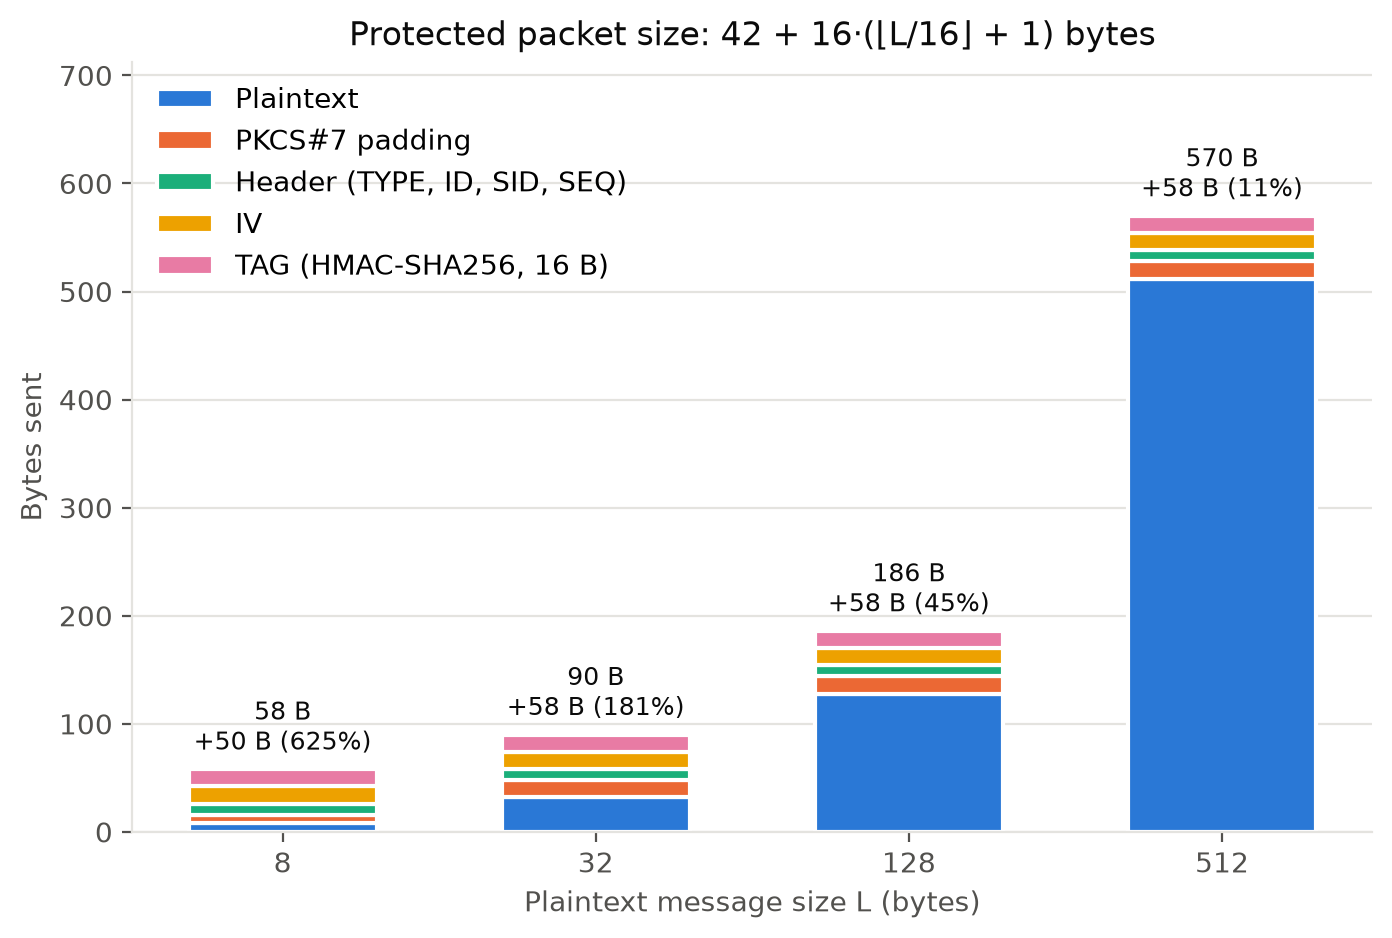
\includegraphics[width=\textwidth]{packet_size.png}
        \caption{Packet size and bytes added.}
    \end{subfigure}\hfill
    \begin{subfigure}[b]{0.49\textwidth}
        \centering
        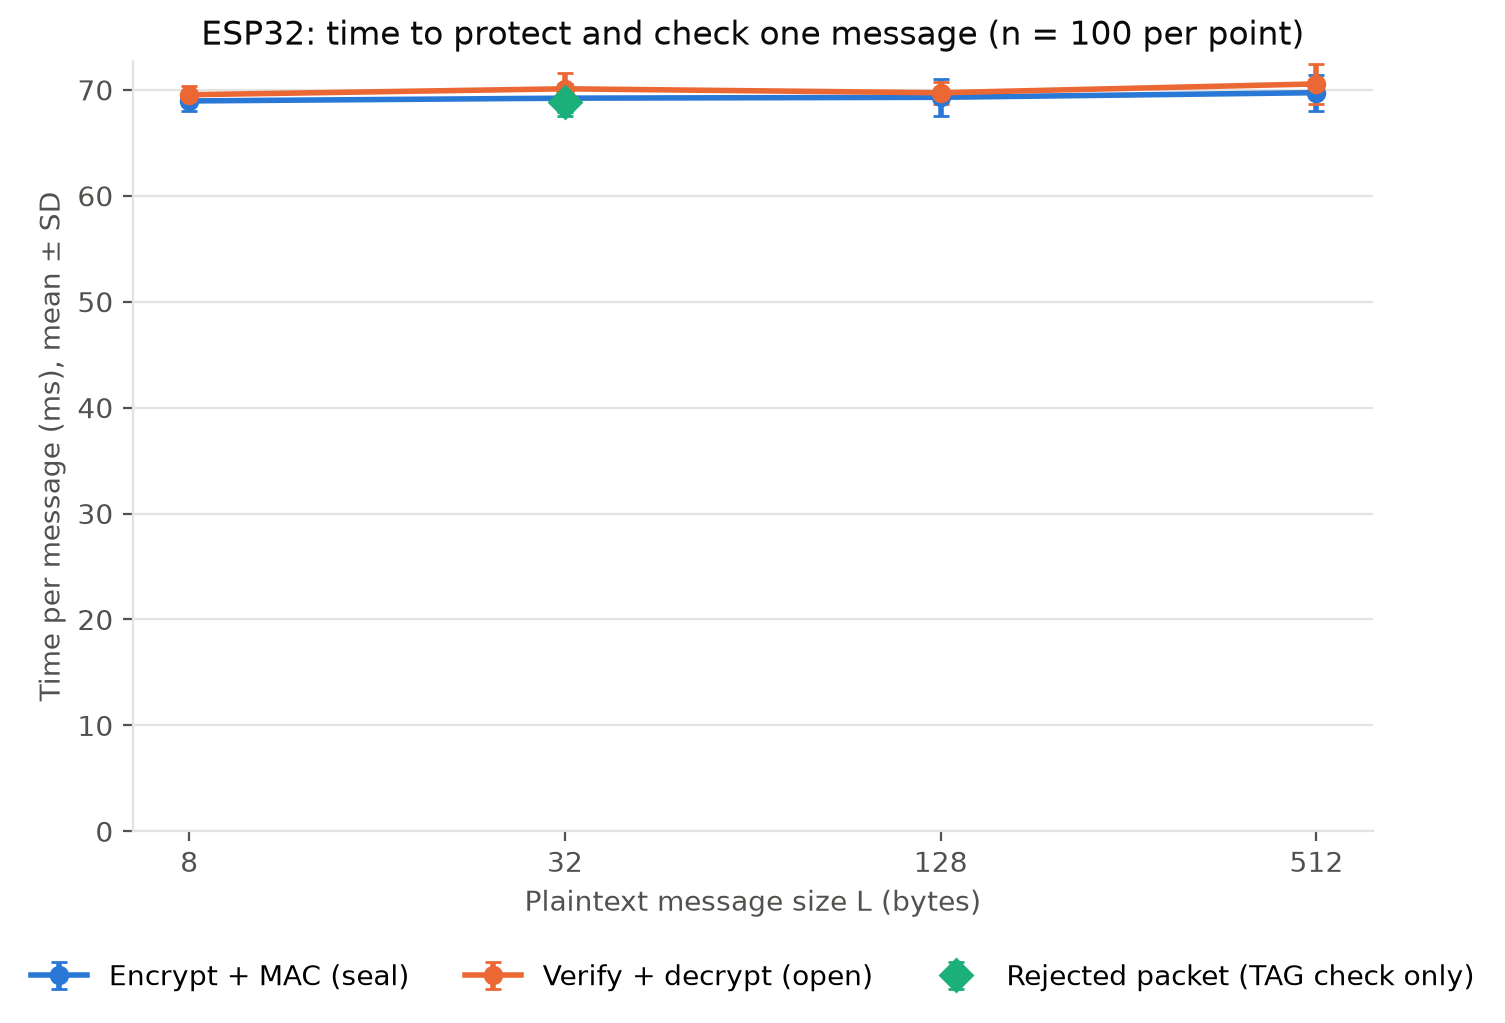
\includegraphics[width=\textwidth]{crypto_time.png}
        \caption{Seal, open, and reject time.}
    \end{subfigure}
    \caption{Cost of protecting one message on the ESP32.}
    \label{fig:sizetime}
\end{figure}

\paragraph{Latency.} The RTT of a protected PING/PONG was
$494.7 \pm 87.3$~ms ($n = 50$, from 375.8 to 659.0~ms), so the one-way latency
is about 247~ms. Each round trip includes two seal and two open operations,
about $2 \times (68.95 + 69.54) \approx 277$~ms, that is, 56\% of the RTT
(\cref{fig:latency}).

\reportfigure[0.95\textwidth]{latency.png}{RTT of 50 protected PING/PONG
messages between the boards, and the share spent on cryptography.}{fig:latency}

\subsection{Security Tests}

The laptop was placed between the boards as the attacker (\texttt{attacker.py}),
so every packet from Alice to Bob went through it. The console captures are in
\cref{app:screens}.

\paragraph{Sniffing.} The attacker forwarded the handshake (HELLO 274~B,
RESPONSE 306~B, CONFIRM 34~B) and the data packet without changing it. Bob
printed the message \texttt{Hey Bob!} correctly, while the attacker only saw
the fields \texttt{TYPE}, \texttt{IDS}, \texttt{SID}, \texttt{SEQ},
\texttt{IV}, \texttt{C}, and \texttt{TAG} as bytes, so the text was not readable
(\cref{fig:normal-bob,fig:normal-sniff}).

\paragraph{Modified ciphertext.} The attacker changed one bit of $C$
(\texttt{f9}~$\rightarrow$~\texttt{f8}) and left the rest of the packet as it
was. Bob printed \texttt{Rejected: TAG} and did not show any message
(\cref{fig:tamperc-attacker,fig:tamperc-bob}).

\paragraph{Replay.} The attacker sent the same valid packet twice. Bob accepted
the first one and printed the message, and then printed
\texttt{Rejected: replay} for the second one, which was identical
(\cref{fig:replay-attacker,fig:replay-bob}).

\paragraph{Forged packet.} The attacker replaced $\mathit{IV}$, $C$, and
$\mathit{TAG}$ with values of its own, without knowing the keys. Bob printed
\texttt{Rejected: TAG} (\cref{fig:forge-attacker,fig:forge-bob}).

% TODO: tamper_tag, mitm and the intruder tests (node.py --id 0x99 and --psk-falsa) are not run yet; add them here only if they are run

\subsection{Discussion}

The main cost of each message is the HMAC and not AES. Rejecting a packet only
computes the HMAC and costs almost the same as a full open, and the time hardly
changes from 8 to 512 bytes. A likely reason is that the \texttt{hmac} module
of MicroPython is written in Python, while AES runs in native code. The
handshake costs about 110 times more than sealing one message because of its
modular exponentiations, but it happens only once per session.

In terms of communication, the protection adds 50 to 58 bytes per message. This
is large for very short messages (625\% for 8 bytes) but small for long ones
(11\% for 512 bytes), and every field is needed for one of the required
properties. Finally, cryptography takes about 56\% of the RTT, and the rest is
the Wi-Fi network. The RTT varies a lot between samples, probably because of the
power saving of the ESP32 Wi-Fi and the phone hotspot, while the cryptographic
times vary by only 1 to 2~ms. Overall, a quarter of a second per direction is
acceptable for short text messages.
% TODO: after the attack tests, add a paragraph that interprets the security results (why each attack was rejected, which check of Listing lst:open stopped it, and why the MITM and the intruder could not obtain a session)

% ============================================================
% 7. KEY QUESTIONS AND DESIGN INSIGHTS
% ============================================================

\section{Key Questions and Design Insights}

This section answers the most important questions about the design and points
out some distinctions that are easy to miss.

\textbf{Is encryption enough to secure the messages?}

No. Encryption hides the content, but it does not stop an attacker from changing or repeating a
packet. For example, flipping one bit of a CBC ciphertext flips the same bit in
the recovered plaintext without any error. Therefore, confidentiality,
integrity, authentication, and freshness must be provided together, which is
why every packet carries a tag, a session identifier, and a sequence number.

\textbf{Why use a PSK if Diffie--Hellman already gives a shared key?} 

Plain DH only guarantees that two parties share a key, not who those parties are. An
attacker in the middle could run one DH exchange with each board. The PSK binds
the exchange to the authorized devices, because only they can compute the HMAC
over the transcript. In addition, MicroPython has no signature library, so a
PSK is the practical way to authenticate the boards.

\textbf{What happens if the PSK is stolen?} 

Past sessions remain secret, because their keys also depend on the ephemeral exponents, which were erased.
However, an attacker with the PSK could impersonate a board in future sessions.
Therefore, a stolen PSK must be replaced on both boards. This is the main
difference between using DHE-PSK and using only a PSK, where a stolen key
would also reveal every recorded session.

\textbf{Why AES-CBC with HMAC instead of AES-GCM?} 

AES-GCM is not available in \texttt{cryptolib}, and implementing it by hand would be custom
cryptography. Encrypt-then-MAC with independent keys reaches the same goal with
standard primitives, as long as the tag is checked before decryption.

\textbf{Why a standard group and a 256-bit exponent?} 

Inventing DH parameters is risky, while \texttt{ffdhe2048} is a published and reviewed
group. Moreover, RFC~7919 asks for an exponent of at least 224 bits for this
group, so 256 bits keeps the security level and makes each exponentiation much
faster on the ESP32.

\textbf{Why is a session identifier needed if the keys change in every session?}

The keys alone would already reject old packets, but only after
computing the HMAC. The $\mathit{SID}$ lets the receiver drop packets from
other sessions at once and report a clear reason for the rejection.

\textbf{What does the system not protect?}

The device IDs travel in clear, so an observer knows who is talking but not what is said. Moreover, the
protocol cannot stop an attacker from blocking packets or from sending many
HELLO messages to keep the board busy with the 7.6~s handshake, which are
denial-of-service attacks that cryptography alone cannot prevent. Finally, a
person with physical access to a board could read the PSK from its flash
memory.

% ============================================================
% 8. CONCLUSIONS
% ============================================================

\section{Conclusions}

We built a secure messaging system between two ESP32 boards that combines
confidentiality, integrity, device authentication, and replay protection in one
protocol, using only standard algorithms and libraries. The session key comes
from an ephemeral DH exchange authenticated with a PSK, and HKDF derives
independent keys and a session identifier. Since MicroPython has no AES-GCM, we
justified and used AES-256-CBC with HMAC-SHA256 in the Encrypt-then-MAC order,
with a tag that covers the whole header and is checked before decryption.

The normal exchange between the two boards works, and the measurements show the
practical cost on the ESP32: about 70~ms and 50 to 58 bytes per message, mostly
due to the HMAC, plus a handshake of about 7.6~s once per session.
% TODO: add the conclusion about the security tests (only after running them): whether every attack was detected and rejected, and whether the unauthorized device was unable to open a session

% ============================================================
% 9. FUTURE WORK
% ============================================================

\section{Future Work}

If a future firmware offers AES-GCM or ChaCha20-Poly1305, the messages could use
a single authenticated encryption mode, and ECDH (for example X25519) would make
the handshake faster and smaller. In addition, a sliding window for
$\mathit{SEQ}$, a limit on HELLO messages, and the flash encryption of the
ESP32 would address the limits described in the previous section.

% ============================================================
% REFERENCES
% ============================================================

\printbibliography[heading=bibintoc]

% ============================================================
% APPENDICES
% ============================================================

\appendix

\section{Additional Material}

\subsection{Screenshots of the Security Tests}
\label{app:screens}

\reportfigure[0.75\textwidth]{Screenshots/01_normal_bob.png}{Normal exchange: Bob receives the message.}{fig:normal-bob}
\reportfigure[0.75\textwidth]{Screenshots/01_normal_sniff.png}{Sniffing: the attacker only sees bytes.}{fig:normal-sniff}
\reportfigure[0.75\textwidth]{Screenshots/02_tamper_c_attacker.png}{Modified ciphertext: the attacker changes one bit of $C$.}{fig:tamperc-attacker}
\reportfigure[0.75\textwidth]{Screenshots/02_tamper_c_bob.png}{Modified ciphertext: Bob rejects the packet (TAG).}{fig:tamperc-bob}
\reportfigure[0.75\textwidth]{Screenshots/04_replay_attacker.png}{Replay: the attacker sends the same packet twice.}{fig:replay-attacker}
\reportfigure[0.75\textwidth]{Screenshots/04_replay_bob.png}{Replay: Bob accepts the first packet and rejects the second.}{fig:replay-bob}
\reportfigure[0.75\textwidth]{Screenshots/05_forge_attacker.png}{Forgery: the attacker replaces IV, $C$, and TAG.}{fig:forge-attacker}
\reportfigure[0.75\textwidth]{Screenshots/05_forge_bob.png}{Forgery: Bob rejects the packet (TAG).}{fig:forge-bob}

% TODO: (optional) add the link to the GitHub repository and to the demo video, once they are final

\end{document}
